\documentclass[11pt]{article}
\usepackage{tikz}
\usetikzlibrary{arrows}
\usetikzlibrary{shapes}
\usepackage{pgfmath}
\usepackage{setspace}
\usepackage{amsmath}
\usepackage{array}
\usepackage{hyperref}
\usepackage{enumerate}
\usepackage{enumitem}
\setlist{noitemsep}
\usepackage{listings}
\lstset{language=python}
\usepackage{makeidx}
\usepackage{verbatim}
\usepackage{datetime}
\usepackage{booktabs}

\setlength{\pdfpageheight}{11in}
\setlength{\textheight}{9in}
\setlength{\voffset}{-1in}
\setlength{\oddsidemargin}{0pt}
\setlength{\marginparsep}{0pt}
\setlength{\marginparwidth}{0pt}
\setlength{\marginparpush}{0pt}
\setlength{\textwidth}{6.5in}

\pagestyle{plain}
\makeindex

\title{Crash Data ML}
\author{Brad Burkman}
\newdateformat{vardate}{\THEDAY\ \monthname[\THEMONTH]\ \THEYEAR}
\vardate
\date{\today}

\begin{document}
\setlength{\parindent}{20pt}
\begin{spacing}{1.2}
\maketitle
\tableofcontents

\section{Reworking the Titanic Notebook}

The Titanic notebook is two years old, and I noticed as I read through it that several times the output had warnings that parts of the code were outdated.  I sometimes got different results.  All of the data prep results were the same.  The differences started when I got to the logistic regression coefficients.  My results on the right, Kaggle's on the left.

\

\begin{tabular}{llr}
\toprule
{} &    Feature &  Correlation \\
\midrule
1 &        Sex &     2.201057 \\
5 &      Title &     0.406027 \\
4 &   Embarked &     0.276628 \\
6 &    IsAlone &     0.185986 \\
7 &  Age*Class &    -0.050260 \\
3 &       Fare &    -0.071665 \\
2 &        Age &    -0.469638 \\
0 &     Pclass &    -1.200309 \\
\bottomrule
\end{tabular}


\vskip -2.5in
\hfill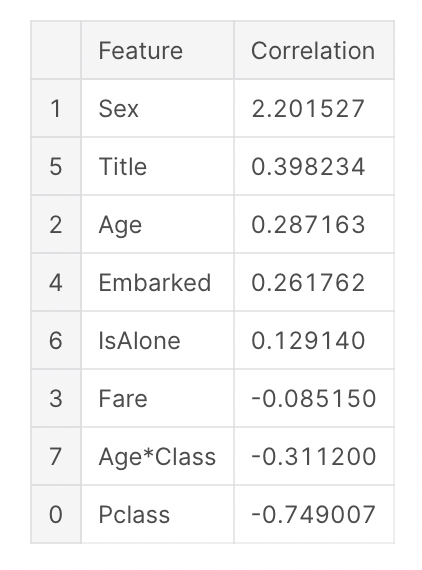
\includegraphics[height=3in]{TitanicLogisticRegressionTable.png}

\newpage

I saw the same differences in the scores of the different models.  

\

\begin{tabular}{llr}
\toprule
{} &                        Model &  Score \\
\midrule
3 &                Random Forest &  86.64 \\
8 &                Decision Tree &  86.64 \\
1 &                          KNN &  84.06 \\
0 &      Support Vector Machines &  82.83 \\
2 &          Logistic Regression &  81.37 \\
7 &                   Linear SVC &  79.46 \\
5 &                   Perceptron &  79.35 \\
4 &                  Naive Bayes &  76.88 \\
6 &  Stochastic Gradient Descent &  76.66 \\
\bottomrule
\end{tabular}


\vskip -2.5in
\hfill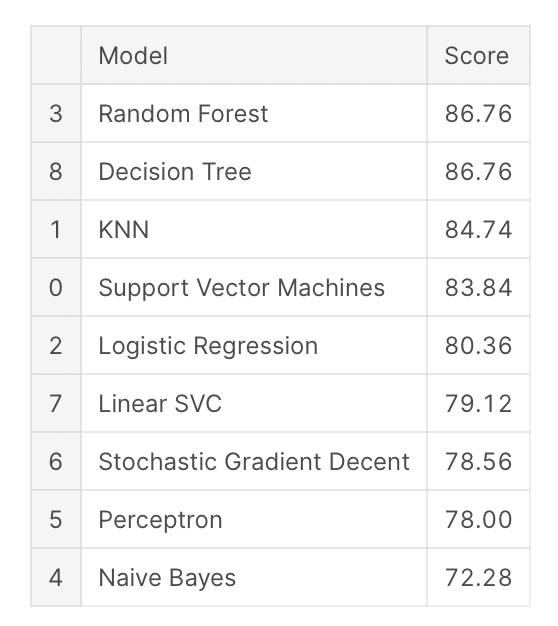
\includegraphics[height=3in]{TitanicModelsTable.png}

\section{Models Scores for Crash Data}

Here are the results of the different models for the Crash Data.  I turned off the SVM calculation because it was just taking too long for a preliminary snapshot.  

\

\begin{tabular}{llr}
\toprule
{} &                        Model &  Score \\
\midrule
3 &                Random Forest &  99.71 \\
8 &                Decision Tree &  99.71 \\
1 &          k-Nearest Neighbors &  99.59 \\
2 &          Logistic Regression &  99.58 \\
5 &                   Perceptron &  99.58 \\
6 &  Stochastic Gradient Descent &  99.58 \\
7 &                   Linear SVC &  99.58 \\
4 &                  Naive Bayes &  95.82 \\
0 &      Support Vector Machines &   0.00 \\
\bottomrule
\end{tabular}




%%%%%%%%%%%%%%%%%%
% Index
\clearpage
\addcontentsline{toc}{section}{Index}
\printindex

%%%%%%%%%%%%%%%%
\end{spacing}
\end{document}

%%%%%%%%%%%%
% Useful tools
%%%%%%%%%

\begin{lstlisting}
Put your code here.
\end{lstlisting}

\lstinputlisting[language=python]{source_filename.py}


